\documentclass[a4paper, 12pt]{article}%тип документа



%отступы
\usepackage[left=1cm,right=1cm,top=1cm,bottom=2cm,bindingoffset=0cm]{geometry}

%%% Работа с русским языком
\usepackage{graphicx}
\usepackage{cmap}                           % поиск в PDF
\usepackage{mathtext} 			 	       % русские буквы в формулах
\usepackage[T2A]{fontenc}               % кодировка
\usepackage[utf8]{inputenc}              % кодировка исходного текста
\usepackage[english,russian]{babel} 
\usepackage{float}
\usepackage{caption}
\usepackage{multirow} 

\usepackage[export]{adjustbox} % локализация и переносы

\usepackage{subfig}% http://ctan.org/pkg/subfig
\usepackage{booktabs}

\usepackage{wrapfig}


%Матеша
\usepackage{amsmath,amsfonts,amssymb,amsthm,mathtools} % AMS
\usepackage{icomma} % "Умная" запятая

%\mathtoolsset{showonlyrefs=true} % Показывать номера только у тех формул, на которые есть \eqref{} в тексте.

%% Шрифты
\usepackage{euscript}	 % Шрифт Евклид
\usepackage{mathrsfs} % Красивый матшрифт

%% Свои команды
\DeclareMathOperator{\sgn}{\mathop{sgn}}

%% Перенос знаков в формулах (по Львовскому)
\newcommand*{\hm}[1]{#1\nobreak\discretionary{}
	{\hbox{$\mathsurround=0pt #1$}}{}}




\author{Гребнев Евгений \\
	Б01-101}
\title{\textbf{Работа 2.1.2 \\ 
		Определение $\frac{C_{p}}{C_{v}}$ методом адиабатического расширения газа}}

\begin{document}
	\maketitle
	\section{Аннотация}
	В данной работе определили $\gamma = \frac{C_{p}}{C_{v}}$ для воздуха с помощью измерения давления в стеклянном сосуде. Измерения производились после адиабатического расширения газа, а затем после нагревания воздуха в сосуде до комнатной температуры. Оценено время установления теплового равновесия после накачивания давления в сосуд. Оценены погрешности полученных величин.
	\section{Теоретические сведения}
	Используемая для опытов экспериментальня установка состоит из стеклянного сосуда А (объёмом около 20 л), снабженного краном К, и U-образного жидкостного манометра, измеряющего избыточное давление газа в сосуде. Схема установки показана на Рис. 1. 
	
	Избыточное давление создаётся с помощью резиновой груши, сосединённой с сосудом трубкой с краном $К_1$.
	
	В начале опыта  в стеклянном сосуде А находится исследуемый газ при комнатной температуре $T_1$ и давлении $P_1$, несколько превышающем атмосферное давление  $P_0$. После открытия крана К, соединяющего сосуд А с атмосферой, давление и температура газа будут понижаться. Это уменьшение температуры приближённо можно считать адиабатическим. 
	
	Для адиабатического процесса можно записать следующее уравнение: 
	
	\begin{equation}\label{mk}
		\left(\dfrac{P_1}{P_2}\right)^{\gamma - 1} = \left(\dfrac{T_1}{T_2}\right)^\gamma , 
	\end{equation} 
	
	где индексом "1" обозначено состояние после повышения давления в сосуде и выравнивания температуры с комнатной, а индексом "2"  $-$ сразу после открытия крана и выравнивания давления с атмосферным. 
	
	После того, как кран К вновь отсоединит сосуд от атмосферы , происходит медленное изохорическое нагревание газа со скоростью, определяемой теплопроводностью стеклянных стенок сосуда. Вместе с ростом температуры растёт и давление газа. З время порядка $\Delta t_T$  (время установления температуры) система достигает равновесия, и установившаяся температура газа $T_3$ становится равной комнатной температуре $T_1$. 
	
	Тогда используя закон Гей-Люссака для изохорического процесса и уравнение \eqref{mk} найдём $\gamma$:
	
	\begin{equation}\label{acc}
		\gamma = \dfrac{\ln(P_1 / P_0)}{\ln (P_1 / P_3)}=\dfrac{\ln(1+\rho g h_1 / P_0)}{\ln(1+\rho g h_1 / P_0)-\ln(1+\rho g h_2 / P_0)}.
	\end{equation}
	\newpage
	Разлагая логарифмы в ряд и пренебрегая членами второго порядка малости получим из \eqref{acc}:
	
	\begin{equation}\label{r}
		\gamma \approx \dfrac{h_1}{h_1 - h_2}.
	\end{equation}
	В работе рассмотрим отличие значения $\gamma$ получаемое из \eqref{acc} и \eqref{r}.
	\begin{figure}[H]
		\centering
		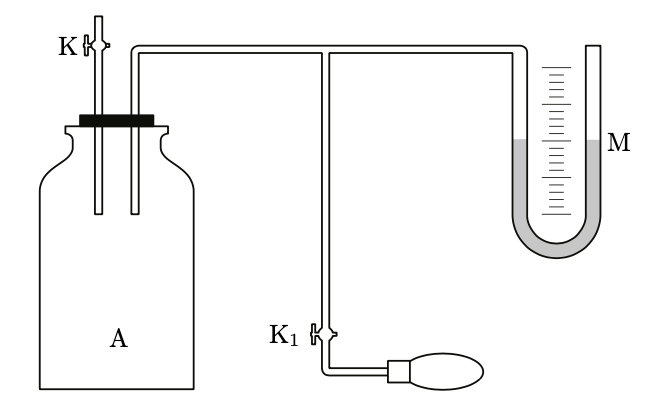
\includegraphics[width=0.6\linewidth]{1}
		\caption{Схема экспериментальной установки}
		\label{fig:1}
	\end{figure}
	\section{Ход работы}
	Определим время установления термодинамического равновесия после накачки воздуха, также проверим систему на герметичность, наблюдая за изменением давления после установления термодинамического равновесия.
	\begin{figure}[H]
		\centering
		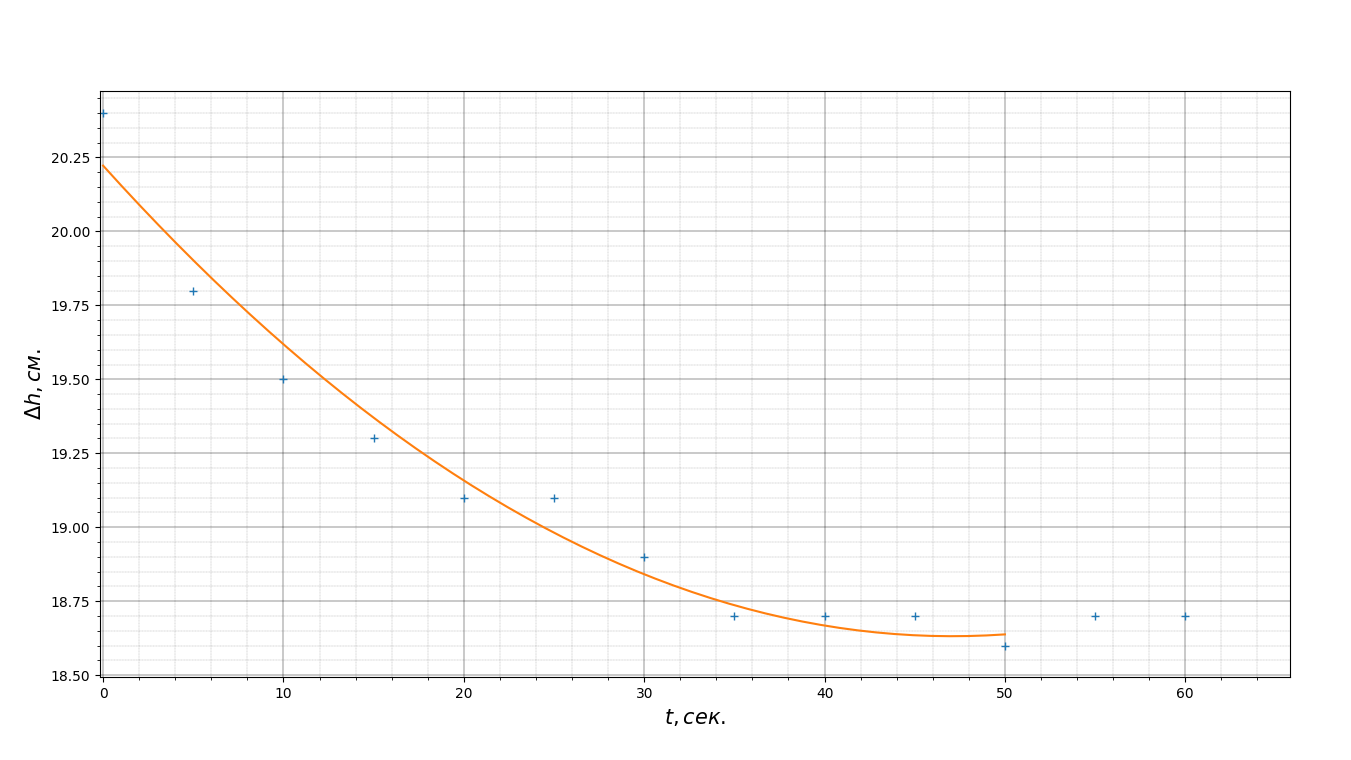
\includegraphics[width=0.82\linewidth]{h_t}
		\caption{Зависимость разности столбиков жидкости от времени}
		\label{fig:ht}
	\end{figure}
	Убедились, что система надежно держит давление, теперь проведем измерения разности высоты в жидкостном манометра перед адиабатическим расширением и после установления теплового равновесия. \textbf{Получили значение времени установления равновесия порядка одной минуты.}
	\begin{table}[H]
		\centering
		\begin{tabular}{|c|c|c|c|c|c|c|}
			\hline
			$\Delta t,~ сек$               & $h_1, ~см$   & $h_2, ~см$  & $\gamma_1\footnotemark[1]~(2), отн.~ед.$ & $\overline{\gamma_1}~(2), отн.~ед.$                      & $\gamma_2\footnotemark[1]~(3), отн.~ед.$ & $\overline{\gamma_2}~(3), отн.~ед.$                   \\ \hline
			\multirow{5}{*}{0.5} & 14.9 & 3.6 & 1.321        & \multirow{5}{*}{$1.324 \pm 0.005$} & 1.319                   & \multirow{5}{*}{$1.321\pm0.005$} \\ \cline{2-4} \cline{6-6}
			& 18.3 & 4.4 & 1.319        &                                 & 1.317                   &                               \\ \cline{2-4} \cline{6-6}
			& 20.5 & 5   & 1.325        &                                 & 1.322                   &                               \\ \cline{2-4} \cline{6-6}
			& 20.1 & 5   & 1.334        &                                 & 1.331                   &                               \\ \cline{2-4} \cline{6-6}
			& 20.3 & 4.9 & 1.321        &                                 & 1.318                   &                               \\ \hline
			\multirow{5}{*}{1}   & 19.7 & 4.7 & 1.316       & \multirow{5}{*}{$1.310\pm 0.011$}   & 1.313                  & \multirow{5}{*}{$1.308\pm0.011$} \\ \cline{2-4} \cline{6-6}
			& 19.9 & 4.9 & 1.330       &                                 & 1.327                  &                               \\ \cline{2-4} \cline{6-6}
			& 13.8 & 3.2 & 1.304       &                                 & 1.302                  &                               \\ \cline{2-4} \cline{6-6}
			& 13.9 & 3.2 & 1.301       &                                 & 1.299                  &                               \\ \cline{2-4} \cline{6-6}
			& 18.3 & 4.2 & 1.301       &                                 & 1.298                  &                               \\ \hline
			\multirow{5}{*}{2}   & 21.3 & 4.6 & 1.278       & \multirow{5}{*}{$1.289\pm 0.008$}   & 1.275                  & \multirow{5}{*}{$1.287\pm 0.009$} \\ \cline{2-4} \cline{6-6}
			& 17.4 & 4   & 1.301       &                                 & 1.299                  &                               \\ \cline{2-4} \cline{6-6}
			& 16.5 & 3.6 & 1.281       &                                 & 1.279                  &                               \\ \cline{2-4} \cline{6-6}
			& 17.7 & 4   & 1.294       &                                 & 1.292                  &                               \\ \cline{2-4} \cline{6-6}
			& 18.7 & 4.2 & 1.292       &                                 & 1.290                  &                               \\ \hline
			\multirow{5}{*}{4}   & 20.1 & 4.2 & 1.27        & \multirow{5}{*}{$1.25\pm 0.06$}     & 1.26                   & \multirow{5}{*}{$1.25\pm 0.06$}   \\ \cline{2-4} \cline{6-6}
			& 19.1 & 3.8 & 1.25        &                                 & 1.25                   &                               \\ \cline{2-4} \cline{6-6}
			& 21.9 & 4.4 & 1.25        &                                 & 1.25                   &                               \\ \cline{2-4} \cline{6-6}
			& 22.5 & 4.5 & 1.25        &                                 & 1.25                   &                               \\ \cline{2-4} \cline{6-6}
			& 16.9 & 3.2 & 1.24        &                                 & 1.23                   &                               \\ \hline
		\end{tabular}
		\caption{Рассчет показателя адиабаты $\gamma$}
	\end{table}
	\footnotetext[1]{В работе при получении формулы (3) мы пренебрегли членами второго порядка при разложении в ряд, из-за этого несомненно возникла некая погрешность. Для понимания ее величины подсчитал $\gamma$ двумя способами: $\gamma_1$ - с использованием точной формулы (2); $\gamma_2$ - с использованием приближения (3).}
	По полученным значениям коэффициента $\gamma$ построим график зависимости $\gamma(\Delta t)$. Аппроксимируя прямой к значению $\Delta t_0 = 0.1~сек.$ получим значение $\gamma$, с учетом минимального отклонения процесса расширения от адиабатического.\\
	Также немаловажным вопросом является оценка полученной величины $\gamma$\footnote[2]{Данный вопрос указан в пункте 3 вывода}, так как она получается путем подстановки в аппроксимирующую прямую. В виду того, что $\gamma = k \Delta t + b$, из логики вычисления погрешности суммы получим:
	$\sigma (\gamma)=\sqrt{\sigma (k \Delta t)^2 + \sigma (b)^2}$. При этом, $\Delta t$ как таковой погрешности в нашем случае не имеет, потому что мы берем его фиксированным значением равным 0.1 сек. По итогу после применения МНК и подстановки погрешностей в формулу получим:$\sigma (\gamma)=0.002~отн.~ед.$\\
	Для последнего интервала $\Delta t$ получили достаточно большую погрешность. Скорее всего это связано со сложностью измерения времени открытия крана. На других интервалах открытие крана представляло непрерывное вращение ручки с разными скоростями, что при достаточной сноровке дает возможность делать схожие по времени интервалы. В последнем же случае приходилось оставлять кран без движения что дает большой разбег значений времени открытия крана.
	\newpage
	\begin{figure}[H]
		\centering
		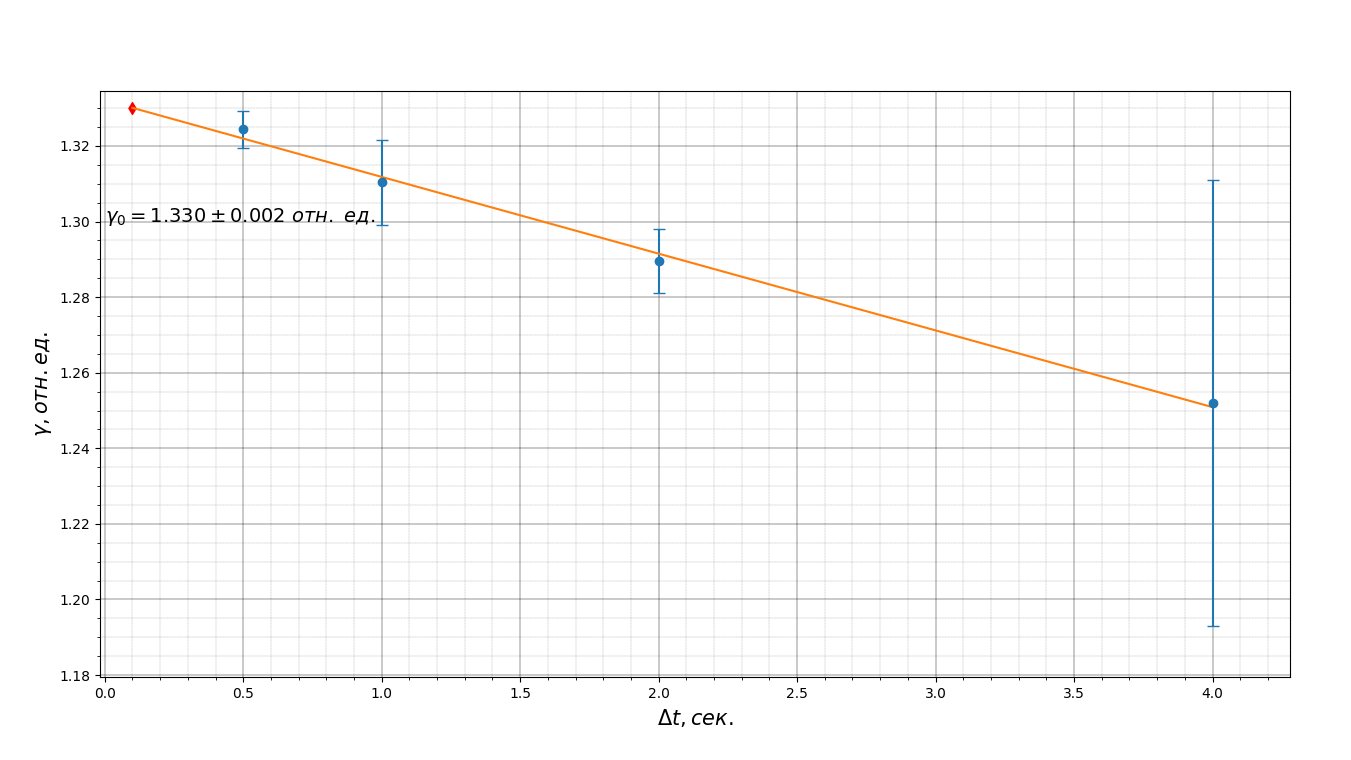
\includegraphics[width=0.95\linewidth]{gamma}
		\caption{Зависимость показателя адиабаты от времени открытия крана}
		\label{fig:gamma}
	\end{figure}
	\section{Вывод}
	1) Оценили показатель адиабаты $\gamma=1.330\pm 0.002$, эталонным для воздуха является значение $\gamma=1.4$, с учетом погрешности значения мы не попадаем в эталонное значение. Однако, в работе не была учтена погрешность определения времени открытия крана, потому что оно является субъективным показателем и невозможно дать какую-либо оценку способности человека отмерять интервалы времени. Также достаточно сложным для определения является момент соединения емкости с атмосферой, так как кран имеет достаточно узкое отверстие.\\
	\textbf{Ввиду вышесказанного можем отметить, что предоставленный метод является лишь способом оценки порядка $\gamma$, а никак не получением ее точного значения. С учетом этого полученное в ходе работы значение является вполне хорошим для оценки $\gamma$.}\\
	2) Оценили время установления теплового равновесия системы. Оно оказалось равным порядка одной минуты.\\
	3)В ходе работы был поставлен важный вопрос об оценке погрешности величины, полученной подстановкой эталонного значения в аппроксимирующую функцию(См. раздел 3 работы).\\ 
\end{document}